\documentclass{isocpp_proposal}
\usepackage{hyperref}
\usepackage{caption}
\usepackage{graphicx}
\usepackage[margin=0.7in]{geometry}



\setsecnumdepth{subsection}
\renewcommand\thesection{\arabic{section}}
\renewcommand\thesubsection{\thesection.\arabic{subsection}}
\setcounter{tocdepth}{2}

\documentnumber{PXXXX}
\date{\today}
\project{Weakening the iterator categories of some standard algorithms}
\replyto{Thibaut Le Jehan $\langle$ lejehan.thibaut@gmail.com $\rangle$}

\usepackage{listings}
\usepackage[usenames, dvipsnames]{color}
\usepackage{changes}

% Definitions and redefinitions of special commands

%%--------------------------------------------------
%% Difference markups
\definecolor{addclr}{rgb}{0,.6,.6}
\definecolor{remclr}{rgb}{1,0,0}
\definecolor{noteclr}{rgb}{0,0,1}

\renewcommand{\added}[1]{\textcolor{addclr}{\uline{#1}}}
\newcommand{\removed}[1]{\textcolor{remclr}{\sout{#1}}}
\renewcommand{\changed}[2]{\removed{#1}\added{#2}}

\newcommand{\nbc}[1]{[#1]\ }
\newcommand{\addednb}[2]{\added{\nbc{#1}#2}}
\newcommand{\removednb}[2]{\removed{\nbc{#1}#2}}
\newcommand{\changednb}[3]{\removednb{#1}{#2}\added{#3}}
\newcommand{\remitem}[1]{\item\removed{#1}}

\newcommand{\ednote}[1]{\textcolor{noteclr}{[Editor's note: #1] }}
% \newcommand{\ednote}[1]{}

\newenvironment{addedblock}
{
\color{addclr}
}
{
\color{black}
}
\newenvironment{removedblock}
{
\color{remclr}
}
{
\color{black}
}

%%--------------------------------------------------
%% Sectioning macros.  
% Each section has a depth, an automatically generated section 
% number, a name, and a short tag.  The depth is an integer in 
% the range [0,5].  (If it proves necessary, it wouldn't take much
% programming to raise the limit from 5 to something larger.)


% The basic sectioning command.  Example:
%    \Sec1[intro.scope]{Scope}
% defines a first-level section whose name is "Scope" and whose short
% tag is intro.scope.  The square brackets are mandatory.
\def\Sec#1[#2]#3{{%
\ifcase#1\let\s=\chapter
      \or\let\s=\section
      \or\let\s=\subsection
      \or\let\s=\subsubsection
      \or\let\s=\paragraph
      \or\let\s=\subparagraph
      \fi%
\s[#3]{#3\hfill[#2]}\label{#2}}}

% A convenience feature (mostly for the convenience of the Project
% Editor, to make it easy to move around large blocks of text):
% the \rSec macro is just like the \Sec macro, except that depths 
% relative to a global variable, SectionDepthBase.  So, for example,
% if SectionDepthBase is 1,
%   \rSec1[temp.arg.type]{Template type arguments}
% is equivalent to
%   \Sec2[temp.arg.type]{Template type arguments}
\newcounter{SectionDepthBase}
\newcounter{scratch}

\def\rSec#1[#2]#3{{%
\setcounter{scratch}{#1}
\addtocounter{scratch}{\value{SectionDepthBase}}
\Sec{\arabic{scratch}}[#2]{#3}}}

\newcommand{\synopsis}[1]{\textbf{#1}}

%%--------------------------------------------------
% Indexing

% locations
\newcommand{\indextext}[1]{\index[generalindex]{#1}}
\newcommand{\indexlibrary}[1]{\index[libraryindex]{#1}}
\newcommand{\indexgram}[1]{\index[grammarindex]{#1}}
\newcommand{\indeximpldef}[1]{\index[impldefindex]{#1}}

\newcommand{\indexdefn}[1]{\indextext{#1}}
\newcommand{\indexgrammar}[1]{\indextext{#1}\indexgram{#1}}
\newcommand{\impldef}[1]{\indeximpldef{#1}implementation-defined}

% appearance
\newcommand{\idxcode}[1]{#1@\tcode{#1}}
\newcommand{\idxhdr}[1]{#1@\tcode{<#1>}}
\newcommand{\idxgram}[1]{#1@\textit{#1}}

%%--------------------------------------------------
% General code style
\newcommand{\CodeStyle}{\ttfamily}
\newcommand{\CodeStylex}[1]{\texttt{#1}}

% Code and definitions embedded in text.
\newcommand{\tcode}[1]{\CodeStylex{#1}}
\newcommand{\techterm}[1]{\textit{#1}\xspace}
\newcommand{\defnx}[2]{\indexdefn{#2}\textit{#1}\xspace}
\newcommand{\defn}[1]{\defnx{#1}{#1}}
\newcommand{\term}[1]{\textit{#1}\xspace}
\newcommand{\grammarterm}[1]{\textit{#1}\xspace}

%%--------------------------------------------------
%% allow line break if needed for justification
\newcommand{\brk}{\discretionary{}{}{}}
%  especially for scope qualifier
\newcommand{\colcol}{\brk::\brk}

%%--------------------------------------------------
%% Macros for funky text
\newcommand{\Rplus}{\protect\hspace{-.1em}\protect\raisebox{.35ex}{\smaller{\smaller\textbf{+}}}}
% \newcommand{\Rplus}{+}
\newcommand{\Cpp}{\mbox{C\Rplus\Rplus}\xspace}
\newcommand{\CppIII}{\Cpp 2003\xspace}
\newcommand{\opt}{{\ensuremath{_\mathit{opt}}}\xspace}
\newcommand{\shl}{<{<}}
\newcommand{\shr}{>{>}}
\newcommand{\dcr}{-{-}}
\newcommand{\exor}{\^{}}
\newcommand{\bigoh}[1]{\ensuremath{\mathscr{O}(#1)}}
% \renewcommand{\tilde}{{\smaller\ensuremath{\sim}}}    % extra level of braces is necessary
\renewcommand{\tilde}{\protect\raisebox{-.5ex}{\larger\textasciitilde}}

%%--------------------------------------------------
%% States and operators
\newcommand{\state}[2]{\tcode{#1}\ensuremath{_{#2}}}
\newcommand{\bitand}{\ensuremath{\, \mathsf{bitand} \,}}
\newcommand{\bitor}{\ensuremath{\, \mathsf{bitor} \,}}
\newcommand{\xor}{\ensuremath{\, \mathsf{xor} \,}}
\newcommand{\rightshift}{\ensuremath{\, \mathsf{rshift} \,}}
\newcommand{\leftshift}[1]{\ensuremath{\, \mathsf{lshift}_#1 \,}}

%% Notes and examples
\newcommand{\EnterBlock}[1]{[\,\textit{#1:}\xspace}
\newcommand{\ExitBlock}[1]{\textit{\,---\,end #1}\,]\xspace}
\newcommand{\enternote}{\EnterBlock{Note}}
\newcommand{\exitnote}{\ExitBlock{note}}
\newcommand{\enterexample}{\EnterBlock{Example}}
\newcommand{\exitexample}{\ExitBlock{example}}

%% Library function descriptions
\newcommand{\Fundescx}[1]{\textit{#1}\xspace}
\newcommand{\Fundesc}[1]{\Fundescx{#1:}}
\newcommand{\required}{\Fundesc{Required behavior}}
\newcommand{\requires}{\Fundesc{Requires}}
\newcommand{\effects}{\Fundesc{Effects}}
\newcommand{\postconditions}{\Fundesc{Postconditions}}
\newcommand{\postcondition}{\Fundesc{Postcondition}}
\newcommand{\preconditions}{\requires}
\newcommand{\precondition}{\requires}
\newcommand{\returns}{\Fundesc{Returns}}
\newcommand{\throws}{\Fundesc{Throws}}
\newcommand{\default}{\Fundesc{Default behavior}}
\newcommand{\complexity}{\Fundesc{Complexity}}
\newcommand{\remark}{\Fundesc{Remark}}
\newcommand{\remarks}{\Fundesc{Remarks}}
\newcommand{\note}{\remark}
\newcommand{\notes}{\remarks}
\newcommand{\realnote}{\Fundesc{Note}}
\newcommand{\realnotes}{\Fundesc{Notes}}
\newcommand{\errors}{\Fundesc{Error conditions}}
\newcommand{\sync}{\Fundesc{Synchronization}}
\newcommand{\implimits}{\Fundesc{Implementation limits}}
\newcommand{\replaceable}{\Fundesc{Replaceable}}
\newcommand{\exceptionsafety}{\Fundesc{Exception safety}}
\newcommand{\returntype}{\Fundesc{Return type}}
\newcommand{\cvalue}{\Fundesc{Value}}
\newcommand{\ctype}{\Fundesc{Type}}
\newcommand{\ctypes}{\Fundesc{Types}}
\newcommand{\dtype}{\Fundesc{Default type}}
\newcommand{\ctemplate}{\Fundesc{Class template}}
\newcommand{\templalias}{\Fundesc{Alias template}}

%% Cross reference
\newcommand{\xref}{\textsc{See also:}\xspace}
\newcommand{\xsee}{\textsc{See:}\xspace}

%% NTBS, etc.
\newcommand{\NTS}[1]{\textsc{#1}\xspace}
\newcommand{\ntbs}{\NTS{ntbs}}
\newcommand{\ntmbs}{\NTS{ntmbs}}
\newcommand{\ntwcs}{\NTS{ntwcs}}
\newcommand{\ntcxvis}{\NTS{ntc16s}}
\newcommand{\ntcxxxiis}{\NTS{ntc32s}}

%% Code annotations
\newcommand{\EXPO}[1]{\textit{#1}}
\newcommand{\expos}{\EXPO{exposition only}}
\newcommand{\exposr}{\expos}
\newcommand{\exposrc}{\expos}
\newcommand{\impdef}{\EXPO{implementation-defined}}
\newcommand{\impdefx}[1]{\indeximpldef{#1}\EXPO{implementation-defined}}
\newcommand{\notdef}{\EXPO{not defined}}

\newcommand{\UNSP}[1]{\textit{\texttt{#1}}}
\newcommand{\unspec}{\UNSP{unspecified}\xspace}
\newcommand{\unspecbool}{\UNSP{unspecified-bool-type}}
\newcommand{\seebelow}{\UNSP{see below}}
\newcommand{\unspecuniqtype}{\UNSP{unspecified unique type}}
\newcommand{\unspecalloctype}{\UNSP{unspecified allocator type}}

%% Double underscore
\newcommand{\unun}{\_\,\_}
\newcommand{\xname}[1]{\unun\,#1}
\newcommand{\mname}[1]{\tcode{\unun\,#1\,\unun}}

%% Ranges
\newcommand{\Range}[4]{\tcode{#1\brk{}#3,\brk{}#4\brk{}#2}\xspace}
\newcommand{\crange}[2]{\Range{[}{]}{#1}{#2}}
\newcommand{\brange}[2]{\Range{(}{]}{#1}{#2}}
\newcommand{\orange}[2]{\Range{(}{)}{#1}{#2}}
\newcommand{\range}[2]{\Range{[}{)}{#1}{#2}}

%% Change descriptions
\newcommand{\diffdef}[1]{\hfill\break\textbf{#1:}\xspace}
\newcommand{\change}{\diffdef{Change}}
\newcommand{\rationale}{\diffdef{Rationale}}
\newcommand{\effect}{\diffdef{Effect on original feature}}
\newcommand{\difficulty}{\diffdef{Difficulty of converting}}
\newcommand{\howwide}{\diffdef{How widely used}}

%% Miscellaneous
\newcommand{\uniquens}{\textrm{\textit{\textbf{unique}}} }
\newcommand{\stage}[1]{\item{\textbf{Stage #1:}}\xspace}
\newcommand{\doccite}[1]{\textit{#1}\xspace}
\newcommand{\cvqual}[1]{\textit{#1}}
\newcommand{\cv}{\cvqual{cv}}
\newcommand{\numconst}[1]{\textsl{#1}\xspace}
\newcommand{\logop}[1]{{\footnotesize #1}\xspace}

%%--------------------------------------------------
%% Environments for code listings.

% We use the 'listings' package, with some small customizations.  The
% most interesting customization: all TeX commands are available
% within comments.  Comments are set in italics, keywords and strings
% don't get special treatment.

\lstset{language=C++,
        basicstyle=\small\CodeStyle,
        keywordstyle=\color{blue},
        stringstyle=\color{red},
        xleftmargin=1em,
        showstringspaces=false,
        commentstyle=\itshape\color{ForestGreen},
        columns=flexible,
        keepspaces=true,
        texcl=true}

% Our usual abbreviation for 'listings'.  Comments are in 
% italics.  Arbitrary TeX commands can be used if they're 
% surrounded by @ signs.
\lstnewenvironment{codeblock}
{
 \lstset{escapechar=@}
 \renewcommand{\tcode}[1]{\textup{\CodeStylex{##1}}}
 \renewcommand{\techterm}[1]{\textit{\CodeStylex{##1}}}
}
{
}

% Permit use of '@' inside codeblock blocks (don't ask)
\makeatletter
\newcommand{\atsign}{@}
\makeatother

%%--------------------------------------------------
%% Indented text
\newenvironment{indented}
{\list{}{}\item\relax}
{\endlist}

%%--------------------------------------------------
%% Library item descriptions
\lstnewenvironment{itemdecl}
{
 \lstset{escapechar=@,
 xleftmargin=0em,
 aboveskip=2ex,
 belowskip=0ex	% leave this alone: it keeps these things out of the
				% footnote area
 }
}
{
}

\newenvironment{itemdescr}
{
 \begin{indented}}
{
 \end{indented}
}


%%--------------------------------------------------
%% Bnf environments
\newlength{\BnfIndent}
\setlength{\BnfIndent}{\leftmargini}
\newlength{\BnfInc}
\setlength{\BnfInc}{\BnfIndent}
\newlength{\BnfRest}
\setlength{\BnfRest}{2\BnfIndent}
\newcommand{\BnfNontermshape}{\small\rmfamily\itshape}
\newcommand{\BnfTermshape}{\small\ttfamily\upshape}
\newcommand{\nonterminal}[1]{{\BnfNontermshape #1}}

\newenvironment{bnfbase}
 {
 \newcommand{\nontermdef}[1]{\indexgrammar{\idxgram{##1}}\nonterminal{##1}:}
 \newcommand{\terminal}[1]{{\BnfTermshape ##1}\xspace}
 \newcommand{\descr}[1]{\normalfont{##1}}
 \newcommand{\bnfindentfirst}{\BnfIndent}
 \newcommand{\bnfindentinc}{\BnfInc}
 \newcommand{\bnfindentrest}{\BnfRest}
 \begin{minipage}{.9\hsize}
 \newcommand{\br}{\hfill\\}
 }
 {
 \end{minipage}
 }

\newenvironment{BnfTabBase}[1]
{
 \begin{bnfbase}
 #1
 \begin{indented}
 \begin{tabbing}
 \hspace*{\bnfindentfirst}\=\hspace{\bnfindentinc}\=\hspace{.6in}\=\hspace{.6in}\=\hspace{.6in}\=\hspace{.6in}\=\hspace{.6in}\=\hspace{.6in}\=\hspace{.6in}\=\hspace{.6in}\=\hspace{.6in}\=\hspace{.6in}\=\kill}
{
 \end{tabbing}
 \end{indented}
 \end{bnfbase}
}

\newenvironment{bnfkeywordtab}
{
 \begin{BnfTabBase}{\BnfTermshape}
}
{
 \end{BnfTabBase}
}

\newenvironment{bnftab}
{
 \begin{BnfTabBase}{\BnfNontermshape}
}
{
 \end{BnfTabBase}
}

\newenvironment{simplebnf}
{
 \begin{bnfbase}
 \BnfNontermshape
 \begin{indented}
}
{
 \end{indented}
 \end{bnfbase}
}

\newenvironment{bnf}
{
 \begin{bnfbase}
 \list{}
	{
	\setlength{\leftmargin}{\bnfindentrest}
	\setlength{\listparindent}{-\bnfindentinc}
	\setlength{\itemindent}{\listparindent}
	}
 \BnfNontermshape
 \item\relax
}
{
 \endlist
 \end{bnfbase}
}

% non-copied versions of bnf environments
\newenvironment{ncbnftab}
{
 \begin{bnftab}
}
{
 \end{bnftab}
}

\newenvironment{ncsimplebnf}
{
 \begin{simplebnf}
}
{
 \end{simplebnf}
}

\newenvironment{ncbnf}
{
 \begin{bnf}
}
{
 \end{bnf}
}

%%--------------------------------------------------
%% Drawing environment
%
% usage: \begin{drawing}{UNITLENGTH}{WIDTH}{HEIGHT}{CAPTION}
\newenvironment{drawing}[4]
{
\newcommand{\mycaption}{#4}
\begin{figure}[h]
\setlength{\unitlength}{#1}
\begin{center}
\begin{picture}(#2,#3)\thicklines
}
{
\end{picture}
\end{center}
\caption{\mycaption}
\end{figure}
}

%%--------------------------------------------------
%% Environment for imported graphics
% usage: \begin{importgraphic}{CAPTION}{TAG}{FILE}

\newenvironment{importgraphic}[3]
{%
\newcommand{\cptn}{#1}
\newcommand{\lbl}{#2}
\begin{figure}[htp]\centering%
\includegraphics[scale=.35]{#3}
}
{
\caption{\cptn}\label{\lbl}%
\end{figure}}

%% enumeration display overrides
% enumerate with lowercase letters
\newenvironment{enumeratea}
{
 \renewcommand{\labelenumi}{\alph{enumi})}
 \begin{enumerate}
}
{
 \end{enumerate}
}

% enumerate with arabic numbers
\newenvironment{enumeraten}
{
 \renewcommand{\labelenumi}{\arabic{enumi})}
 \begin{enumerate}
}
{
 \end{enumerate}
}

%%--------------------------------------------------
%% Definitions section
% usage: \definition{name}{xref}
%\newcommand{\definition}[2]{\rSec2[#2]{#1}}
% for ISO format, use:
\newcommand{\definition}[2]
 {\hfill\vspace{.25ex plus .5ex minus .2ex}\\
 \addtocounter{subsection}{1}%
 \textbf{\thesubsection\hfill\relax[#2]}\\
 \textbf{#1}\label{#2}\\
 }
 
 %% adopted from standard's layout.tex
 \newcounter{Paras}
\counterwithin{Paras}{chapter}
\counterwithin{Paras}{section}
\counterwithin{Paras}{subsection}
\counterwithin{Paras}{subsubsection}
\counterwithin{Paras}{paragraph}
\counterwithin{Paras}{subparagraph}

 \makeatletter
\def\pnum{\addtocounter{Paras}{1}\noindent\llap{{%
  \scriptsize\raisebox{.7ex}{\arabic{Paras}}}\hspace{\@totalleftmargin}\quad}}
\makeatother


%%--------------------------------------------------
%% Green and red for added/removed text

\definecolor{LightGreen}{RGB}{160, 255, 160}
\definecolor{LightRed}{RGB}{151, 28, 85}


% Configure escaping in item declarations
\lstset{
    escapeinside={(*@}{@*)},
}

\begin{document}
\maketitle

\section{Introduction}

This paper proposes to weaken the iterator categories of several standard library generic algorithms to reflect the advances in made in the realm of algorithms. Such changes were already proposed in the Palo Alto report \cite{N3351} but were later dropped in the Ranges TS \cite{N4560}, stating that such changes would be best done in a separate proposal (clause B.2.6). Most of the changes are based on the algorithmic research done since the standardization of the standard algorithms, and notably on the advances reported in Stepanov and McJones' \emph{Elements of Programming} \cite{EOP}.

\vspace{0.3cm}

This proposal includes the wording for the new versions of the algorithms, as well as updated complexities. It also includes some further comments and benchmarks to demonstrate that weakening the iterator categories of these algorithms is worth it. We propose to make the following algorithms work with forward iterators:

\begin{itemize}
\item \tcode{std::inplace\_merge}
\item \tcode{std::sort}
\item \tcode{std::stable\_sort}
\end{itemize}

\section{Motivation and Scope}

Currently, the functions \tcode{std::sort} and \tcode{std::stable\_sort} only work with random-access iterators, making it possible to sort classes such as \linebreak \tcode{std::vector}, \tcode{std::deque} and \tcode{std::string}, but not the standard library containers \tcode{std::list} and \tcode{std::forward\_list}, which respectively provide bidirectional and forward iterators. However, both of them have a member function \tcode{sort} to perform the job, even though sorting through a member function is hardly a generic approach. Even the recent C++ Core Guidelines \cite{CppCoreGuidelines} agree on that:

\begin{quotation}
It is probably a dumb idea to define a \tcode{sort} as a member function of a container, but it is not unheard of and it makes a good example of what not to do.
\end{quotation}

That said, \tcode{std::list::sort} and \tcode{std::forward\_list::sort} have a reason to exist: these algorithms can make more assumptions knowing that they work on list data structures, allowing for a  $\mathcal{O}(\log{} n)$ space complexity instead of a  $\mathcal{O}(n)$ one for a classic mergesort. Moreover, these functions don't invalidate the iterators and even work when the stored elements are not moveable. These improvements are due to the ability that lists have to relink nodes instead of moving values around. However, this approach is hardly generic: it only allows to sort full lists instead of arbitrary pairs of iterators, and it forces to add a corresponding member function \tcode{sort} to custom classes wrapping a list and offering an iterator interface. Weakening the iterator categories of the generic sorting algorithms would solve both of these problems.

\vspace{0.3cm}

To add to the confusion, the standard mandates that the member functions \tcode{std::list::sort} and \tcode{std::forward\_list::sort} are stable even though the name does not reflect the guarantee (while \tcode{std::stable\_sort} makes it clear that the algorithm is stable).

\vspace{0.3cm}

Basically, we would like to be able to sort pairs of forward, bidirectional and random-access iterators through a common algorithm interface. The algorithm \tcode{std::inplace\_merge} is often a building block of \tcode{std::stable\_sort} and clearly influences its complexity guarantees; therefore it makes sense to weaken its iterator category to forward iterators too (algorithms exist).

\section{Discussion}

\subsection{Complexity of \tcode{std::sort}}

Some versions of quicksort work reasonably well with forward iterators with an average $\mathcal{O}(n \log{} n)$ complexity but have a $\mathcal{O}(n^2)$ worst case complexity. A simple mergesort may always have a $\mathcal{O}(n \log{} n)$ complexity, but it requires $\mathcal{O}(n)$ auxiliary memory. The most efficient sorting algorithms such as introsort \cite{introsort} and pattern-defeating quicksort \cite{pdqsort} only work with random-access iterators because they need to fall back to a heapsort in order to avoid the quadratic behavior of quicksort.

\vspace{0.3cm}

We think that the right approach to this  problem is to only guarantee an $\mathcal{O}(n \log{} n)$ average complexity for forward and bidirectional iterators, and either no worst case complexity or a $\mathcal{O}(n^2)$ worst case complexity. In C++03, \tcode{std::sort} has no worst case complexity guarantee, before efficient algorithms with an $\mathcal{O}(n \log{} n)$ worst case complexity were discovered. A simple mergesort has a $\mathcal{O}(n \log{} n)$ worst case complexity for forward and bidirectional iterators, but it requires additional memory and \tcode{std::sort} has an history of not using much additional memory to sort a collection.

\subsection{Complexity of \tcode{std::stable\_sort}}

The current complexity mandated for \tcode{std::stable\_sort} is described as follows: 

\begin{quotation}
It does at most $N \log{}^2 (N)$ (where \tcode{$N$ == last - first}) comparisons; if enough extra memory is available, it is  $N \log{} (N)$.
\end{quotation}

This description more or less corresponds to a trivial mergesort implementation using \tcode{std::inplace\_merge} to perform the merge operation. Since \tcode{std::inplace\_merge} accepts bidirectional iterators, it is easy to make \linebreak \tcode{std::stable\_sort} work with bidirectional iterators as well, with the exact same complexity guarantees as with random-access iterators.

\vspace{0.3cm}

In-place merge algorithms also exist for forward iterators, with or without using a temporary buffer, even though the standard library function \tcode{std::inplace\_merge} is only guaranteed to work with bidirectional iterators. In \emph{Elements of Programming} \cite{EOP}, there is an implementation of an in-place merge algorithm working with forward iterators which adapts to the available memory. That algorithm runs in $\mathcal{O}(n)$ time hen enough memory is available and in $\mathcal{O}(n \log{} n)$ if no additional memory is available, which means that a mergesort for forward iterators can run in $\mathcal{O}(n \log{} n)$ or $\mathcal{O}(n \log{}^2 n)$ time depending on the available memory, which corresponds to the current complexity of \tcode{std::stable\_sort} for random-access iterators.

\subsection{Benefits of \tcode{sort} member functions}

\tcode{std::list::sort} and \tcode{std::forward\_list::sort} can be more efficient than general-purpose stable sorting algorithms for forward and bidirectional iterators; this is due to the fact that they can relink the list's nodes instead of moving or swapping the values. One could say that having general-purpose sorting algorithms for bidirectional and forward iterators might encourage to use them on these data structures while they might be less efficient than the member functions.

\vspace{0.3cm}

While having \tcode{std::sort} call \tcode{std::list::sort} when given list iterators would be an interesting idea, the standard generic algorithms are not allowed to alter the containers, and relinking nodes clearly counts as altering the list; therefore, relinking nodes when using generic algorithms is not a legal optimization.

\vspace{0.3cm}

To make sure that using a generic version of \tcode{std::sort} on lists wouldn't incur a big performance loss, we implemented some basic sorting algorithms for bidirectional and forward iterators and did some benchmarks. While our implementations are not as refined as the ones typically found in standard library implementations, the benchmarks show that some generic sorting algorithms are not orders of magnitude slower than \tcode{std::list::sort} and perform rather well (see the \hyperref[App:Benchmarks]{appendix}). Our sorting algorithms for forward iterators are not that good compared to \tcode{std::forward\_list::sort} but we believe that good implementations might perform better than ours. Also, note that the benchmarks have been performed with lists of integers and that node relinking might always outperform our sorting algorithms for objects that are expensive to move around.

\pagebreak

\subsection{Parallel sorting algorithms}

This proposal focuses on the sequential algorithms from the standard library header \tcode{<algorithm>}, but we believe that the parallel algorithms from the Parallelism TS \cite{N4507} could be other targets for such a change. This paper does not propose to weaken the iterator categories of the corresponding algorithms in the Parallelism Ts, but we encourage people to check whether it can be done and to analyze the resulting algorithmic complexities.

\subsection{Range algorithms}

The Ranges TS \cite{N4560} is yet another obvious target for such a change. It currently redefines \tcode{std::sort} and \tcode{std::stable\_sort} so that they can work with an \tcode{[iterator, sentinel)} pair or a full iterable.

\vspace{0.3cm}

No change was made to the required iterator category by the Ranges TS; random-access iterators are still required for every algorithm we propose to change. Our proposal and the ranges one might be considered at the same time, in which case we also propose to make the new overloads of \tcode{std::sort}, \tcode{std::stable\_sort} and \tcode{std::inplace\_merge} use the \tcode{ForwardIterator} concept instead of the \tcode{RandomAccessIterator} one, and the \tcode{ForwardIterable} concept instead of the \tcode{RandomAccessIterable} one.

\section{Proposed wording}

\textbf{25.4.1.1 \tcode{sort} [sort]}

\begin{lstlisting}
template<class (*@\deleted{RandomAccessIterator}\added{ForwardIterator}@*)>
  void sort((*@\deleted{RandomAccessIterator}\added{ForwardIterator}@*) first,
            (*@\deleted{RandomAccessIterator}\added{ForwardIterator}@*) last);

template<class (*@\deleted{RandomAccessIterator}\added{ForwardIterator}@*),
    class Compare>
  void sort((*@\deleted{RandomAccessIterator}\added{ForwardIterator}@*) first,
            (*@\deleted{RandomAccessIterator}\added{ForwardIterator}@*) last,
            Compare comp);
\end{lstlisting}

\begin{itemdescr}
\pnum
\emph{Effects:} Sorts the elements in the range \tcode{[first, last)}.

\pnum
\emph{Requires:} \deleted{\tcode{RandomAccessIterator}}\added{\tcode{ForwardIterator}} shall satisfy the requirements of
\tcode{ValueSwappable}~(17.6.3.2). The type of \tcode{*first} shall satisfy the requirements of \tcode{MoveConstructible} (Table~20) and of \linebreak \tcode{MoveAssignable} (Table~22).

\pnum
\emph{Complexity:} $\mathcal{O}(N \log{} N)$ (where \tcode{$N$ == last - first}) comparisons \added{on average. At most $\mathcal{O}(N \log{} N)$ comparisons if \tcode{ForwardIterator} additionally satisfies the requirements of \tcode{RandomAccessIterator} \linebreak (Table~110)}.
\end{itemdescr}

\newpage

\textbf{25.4.1.2 \tcode{stable\_sort} [stable.sort]}

\begin{lstlisting}
template<class (*@\deleted{RandomAccessIterator}\added{ForwardIterator}@*)>
  void stable_sort((*@\deleted{RandomAccessIterator}\added{ForwardIterator}@*) first,
                   (*@\deleted{RandomAccessIterator}\added{ForwardIterator}@*) last);

template<class (*@\deleted{RandomAccessIterator}\added{ForwardIterator}@*),
    class Compare>
  void stable_sort((*@\deleted{RandomAccessIterator}\added{ForwardIterator}@*) first,
                   (*@\deleted{RandomAccessIterator}\added{ForwardIterator}@*) last,
                   Compare comp);
\end{lstlisting}

\begin{itemdescr}
\pnum
\emph{Effects:} Sorts the elements in the range \tcode{[first, last)}.

\pnum
\emph{Requires:} \deleted{\tcode{RandomAccessIterator}}\added{\tcode{ForwardIterator}} shall satisfy the requirements of
\tcode{ValueSwappable}~(17.6.3.2). The type of \tcode{*first} shall satisfy the requirements of \tcode{MoveConstructible} (Table~20) and of \linebreak \tcode{MoveAssignable} (Table~22).

\pnum
\emph{Complexity:} It does at most $N \log{}^2 (N)$ (where \tcode{$N$ == last - first}) comparisons; if enough extra memory is available, it is $N \log{}(N)$.

\pnum
\emph{Remarks:} Stable~(17.6.5.7).
\end{itemdescr}

\textbf{25.4.4 Merge}

\begin{lstlisting}
template<class (*@\deleted{BidirectionalIterator}\added{ForwardIterator}@*)>
  void inplace_merge((*@\deleted{BidirectionalIterator}\added{ForwardIterator}@*) first,
                     (*@\deleted{BidirectionalIterator}\added{ForwardIterator}@*) middle,
                     (*@\deleted{BidirectionalIterator}\added{ForwardIterator}@*) last);

template<class (*@\deleted{BidirectionalIterator}\added{ForwardIterator}@*),
    class Compare>
  void inplace_merge((*@\deleted{BidirectionalIterator}\added{ForwardIterator}@*) first,
                     (*@\deleted{BidirectionalIterator}\added{ForwardIterator}@*) middle,                    
                     (*@\deleted{BidirectionalIterator}\added{ForwardIterator}@*) last,
                     Compare comp);
\end{lstlisting}

\begin{itemdescr}
\pnum
\emph{Effects:} Merges two sorted consecutive ranges \tcode{[first, middle)} and \tcode{[middle, last)}, putting the result of the merge into the range \tcode{[first, last)}. The resulting range will be in non-decreasing order; that is, for every iterator \tcode{i} in \tcode{[first, last)} other than \tcode{first}, the condition \linebreak \tcode{*i < *(i - 1)} or, respectively, \tcode{comp(*i, *(i - 1))} will be false.

\pnum
\emph{Requires:} The ranges \tcode{[first, middle)} and \tcode{[middle, last)} shall be sorted with respect to \tcode{operator<} or \tcode{comp}. \deleted{\tcode{BidirectionalIterator}} \added{\tcode{ForwardIterator}} shall satisfy the requirements of \tcode{ValueSwappable} (17.6.3.2). The type of \tcode{*first} shall satisfy the requirements of \linebreak \tcode{MoveConstructible} (Table~20) and of \tcode{MoveAssignable} (Table~22).

\pnum
\emph{Complexity:} When enough additional memory is available, \tcode{(last - first) - 1} comparisons. If no additional memory is available, an algorithm with complexity $N \log{} (N)$ (where \tcode{$N$} is equal to \tcode{last - first}) may be used.

\pnum
\emph{Remarks:} Stable~(17.6.5.7).
\end{itemdescr}

\section{Conclusion}

The standard library should make state-of-the-art algorithms available when those ones are easy enough to implement and strive to weaken the iterator categories of these algorithms when doing so occurs no obvious drawback. Sorting algorithms and related algorithms have been studied in depth over the course of the years, and the algorithms discovered since the birth of the standard library allow to efficiently implement some standard algorithms with weakened iterator categories, which is what we propose to standardize with this paper.

\section{Acknowledgments}

Thanks to Walter E. Brown for the thorough review of this proposal and for offering to present it.

\newpage
\begin{appendices}
\section*{Appendix: Benchmarks} \label{App:Benchmarks}
\addcontentsline{toc}{section}{\protect\numberline{}Appendix: Benchmarks}

In order to check whether \tcode{std::sort} and \tcode{std::stable\_sort} overloads for forward and bidirectional iterators would be fast enough for production uses, or abysmally slower than \tcode{std::list::sort} and \tcode{std::forward\_list::sort}, we implemented a median-of-9 quicksort, and a mergesort relying on the \tcode{std::inplace\_merge} overload for forward iterators based on the algorithms described in \emph{Elements of Programming} \cite{EOP}. The code of the algorithms and of the benchmarks can be found in the library cpp-sort \cite{cpp-sort}. The benchmarks were generated on Windows with MinGW g++ 5.3 and the options \tcode{-std=c++14 -O3 -march=native}, and thus use the list sorting functions from libstdc++.

\begin{figure}[h]
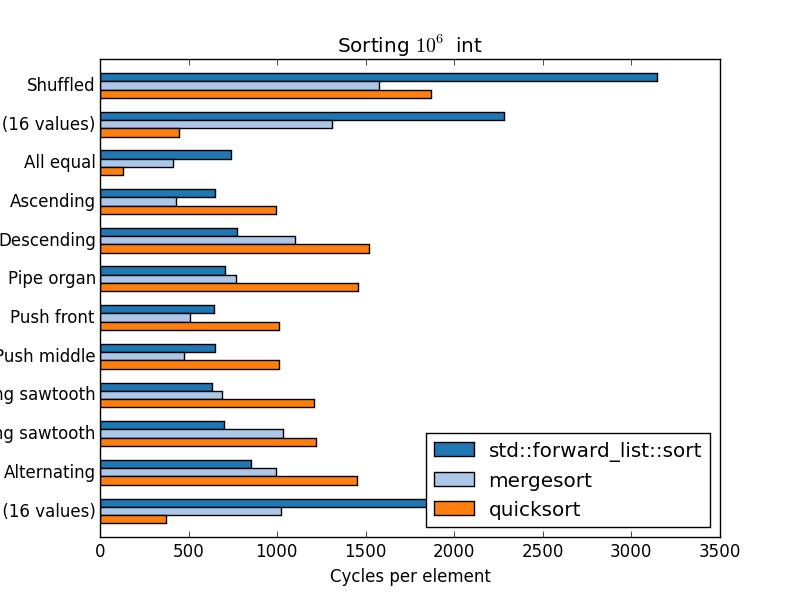
\includegraphics[width=\textwidth]{forward-list-int.png}
\end{figure}

The benchmarks sort collections of one million elements with the given sorting algorithms and compare the running times. Several patterns are benchmarked to display how the different sorting algorithms adapt to the patterns present in the collections to sort. It is also worth noting that mergesort has different implementations for forward and bidirectional iterators: the one used for forward iterators builds upon a the in-place merge algorithm from \emph{Elements of Programming} and uses a few tricks to allocate less memory, hence the good performance on almost sorted data. The one used for bidirectional iterators builds upon the \tcode{std::inplace\_merge} implementation from libc++ but its implementation is rather trivial, we didn't make efforts to optimize it as much as the forward iterators one (the implementation of the bidirectional version almost corresponds to the textbook implementation of a mergesort).

\begin{figure}[h]
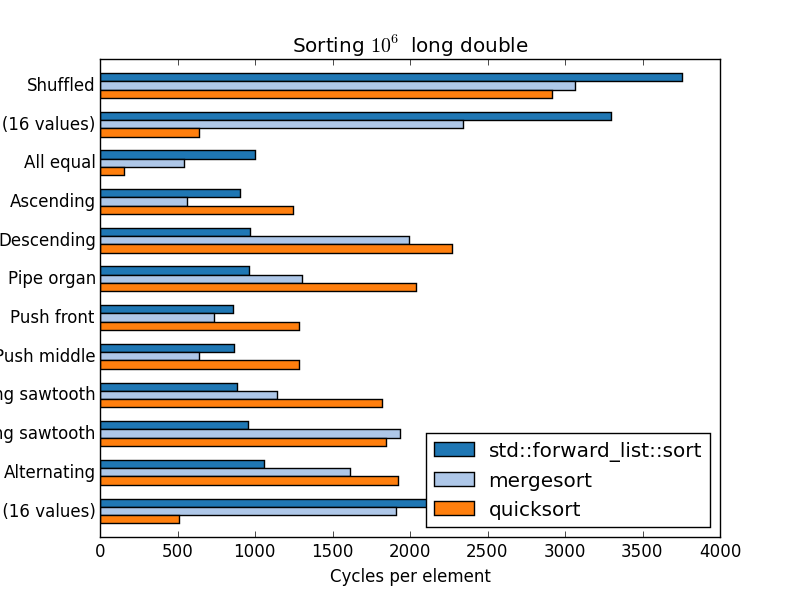
\includegraphics[width=\textwidth]{forward-list-long-double.png}
\end{figure}

For the sake of simplicity, we only benchmarked collections of \tcode{int} and \tcode{long double} values. Be it for forward or bidirectional iterators, there is no clear winner: the \tcode{sort} method of the lists seem to always be the slowest when the values are "truly" random, but it seems to adapt more smoothly to patterns than the other algorithms -- except \emph{Alternating (16 values)}. Mergesort is pretty good for \tcode{std::forward\_list} when the collection is almost sorted, but its bidirectional version is almost always the slowest one; it probably has to do with the fact that the implementation is not as optimized as the forward iterator one, as mentioned in the previous paragraph. Quicksort isn't good with patterns, but it is by far the fastest algorithm when the collection to sort only contains a handful of different values. Also, note that quicksort can degrade to $\mathcal{O}(n \log{}^2 n)$ even though none of the benchmarked patterns trigger this behavior.

\newpage

\begin{figure}[h]
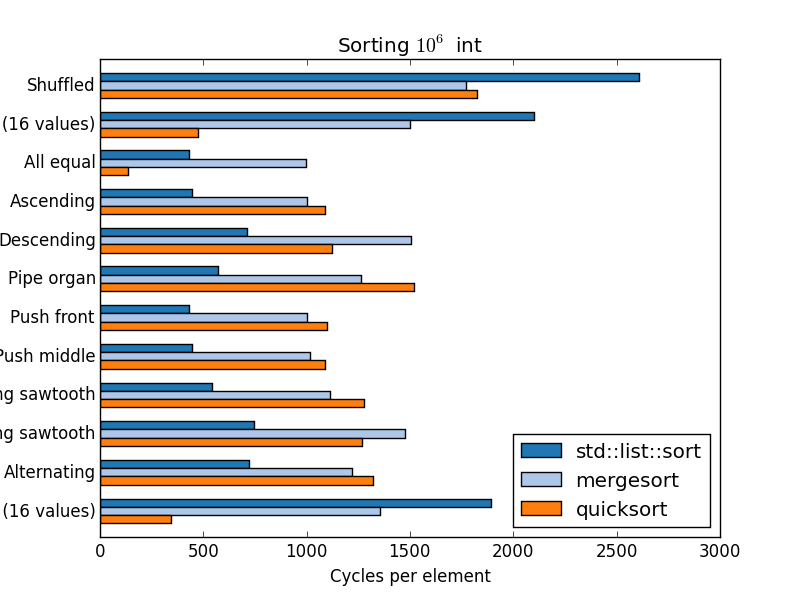
\includegraphics[width=\textwidth]{list-int.png}
\end{figure}

To sum up: the major difference between the algorithms used to sort forward and bidirectional iterators is the performance difference of mergesort for some patterns, which is mostly due to the different implementations of the algorithm. The difference between sorting \tcode{int} and \tcode{long double} values isn't obvious, but the \tcode{sort} method of \tcode{std::list} and \tcode{std::forward\_list} is comparatively better, especially for \tcode{std::list}. Due to the way lists sort themselves, we expect that the \tcode{sort} methods become better and better compared to the other algorithms when the size of the objects and the cost of a move or swap operation grows.

\begin{figure}[h]
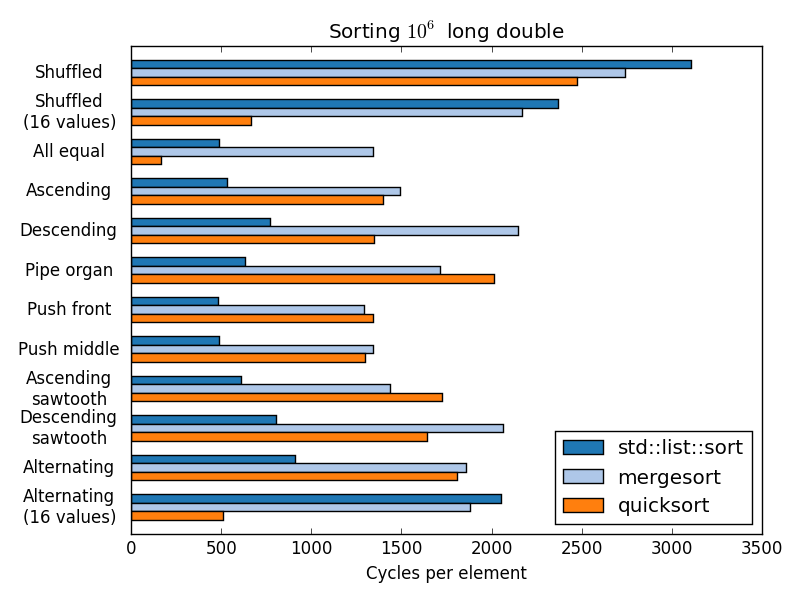
\includegraphics[width=\textwidth]{list-long-double.png}
\end{figure}


\end{appendices}

\newpage
\bibliographystyle{IEEEtran}
\bibliography{biblio}

\end{document}  
